\documentclass[a4paper,14pt]{article}

\usepackage{comment} % Para comentar várias linhas ao mesmo tempo

%matemática
\usepackage{amsmath}
\usepackage{amssymb}

%diagramação
\usepackage{extsizes}
\everymath{\displaystyle}
\usepackage{geometry}
\usepackage{fancyhdr}
\usepackage{multicol}
\usepackage{graphicx}
\usepackage[brazil]{babel}
\usepackage[shortlabels]{enumitem}
\usepackage{cancel}
\usepackage{textcomp}
\usepackage{tcolorbox}

%tabelas
\usepackage{array} % Para melhor formatação de tabelas
\usepackage{longtable}
\usepackage{booktabs}  % Para linhas horizontais mais bonitas
\usepackage{float}   % Para usar o modificador [H]
\usepackage{caption} % Para usar legendas em tabelas
\usepackage{wrapfig} % Para usar tabelas e figuras flutuantes
\usepackage{xcolor} % Para cores do fundo de tabelas
\usepackage{colortbl} % Para cores do fundo de tabelas

%tikzpicture
\begin{comment}
	\usepackage{tikz}
	\usepackage{scalerel}
	\usepackage{pict2e}
	\usepackage{tkz-euclide}
	\usetikzlibrary{calc}
	\usetikzlibrary{patterns,arrows.meta}
	\usetikzlibrary{shadows}
	\usetikzlibrary{external}
\end{comment}


%pgfplots
\usepackage{pgfplots}
\pgfplotsset{compat=newest}
\usepgfplotslibrary{statistics}
\usepgfplotslibrary{fillbetween}

%colours
\usepackage{xcolor}



\columnsep=2cm
\hoffset=0cm
\textwidth=8cm
\setlength{\columnseprule}{.1pt}
\setlength{\columnsep}{2cm}
\renewcommand{\headrulewidth}{0pt}
\geometry{top=1in, bottom=1in, left=0.7in, right=0.5in}

\pagestyle{fancy}
\fancyhf{}
\fancyfoot[C]{\thepage}

\begin{document}
	
	\noindent\textbf{6FMA115 - Matemática} 
	
	\begin{center}Escrevendo porcentagens como decimais (Versão estudante)
	\end{center}
	
	\noindent\textbf{Nome:} \underline{\hspace{10cm}}
	\noindent\textbf{Data:} \underline{\hspace{4cm}}
	
	%\section*{Questões de Matemática}
	
	\begin{multicols}{2}
		\noindent Para transformar uma porcentagem em decimal, dividimos o numeral antes do símbolo \% por 100, ou seja, a vírgula se desloca duas casas para a esquerda. \\
		Para transformar um decimal em porcentagem, multiplicamos o número por 100, ou seja, deslocamos a vírgula duas casas para a direita e acrescentamos o símbolo \%. \\
		Resumindo: \\
		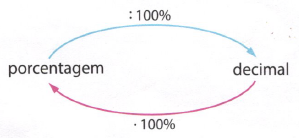
\includegraphics[width=1\linewidth]{6FMA115_imagens/imagem1}
		\noindent\textsubscript{--------------------------------------------------------------------------------------------------------------------------------------------------------------}
		\begin{enumerate} 
			\item Escreva na forma decimal:
			\begin{enumerate}[a)]
				\item 74\% \\\\\\\\
				\item 2\% \\\\\\\\
				\item 30\% \\\\\\\\
				\item 2,15\% \\\\\\\\
				\item 4,7\% \\\\\\\\
				\item 60,2\% \\\\\\\\
			\end{enumerate}
			\item Escreva na forma de porcentagem:
			\begin{enumerate}[a)]
				\item 0,29 \\\\\\\\
				\item 2,32 \\\\\\\\
				\item 0,8 \\\\\\\\
				\item 0,0006 \\\\\\\\
				\item 0,05 \\\\\\\\
				\item 4 \\\\\\\\
			\end{enumerate}
			\item Usando a forma decimal da porcentagem, calcule:
			\begin{enumerate}[a)]
				\item 20\% de 230. \\\\\\\\
				\item 80\% de 35. \\\\\\\\
				\item 50\% de 26. \\\\\\\\
				\item 40\% de 90. \\\\\\\\
			\end{enumerate}
			\item Quando multiplicamos um número por 0,75, que porcentagem desse número estamos calculando? \\\\\\\\
			\item Dado um retângulo, multiplicamos os seus lados por 0,6, obtendo um novo retângulo.
			\begin{enumerate}[a)]
				\item Os lados do novo retângulo representam que porcentagem dos lados do retângulo original? \\\\\\\\\\\\\\\\
				\item Sabe-se que a área de um retângulo de lados $a$ e $b$ é igual a $a \cdot b$. \\
				Com relação ao item $a$, a área do novo retângulo representa que porcentagem da área do retângulo original? \\\\\\\\\\\\\\\\\\
			\end{enumerate}
			%18 a 22
			\item Escreva na forma decimal:
			\begin{enumerate}[a)]
				\item 8\% \\\\\\\\
				\item 13\% \\\\\\\\
				\item 57\% \\\\\\\\
				\item 106\% \\\\\\\\
				\item 97,8\% \\\\\\\\
				\item 0,12\% \\\\\\\\
			\end{enumerate}
			\item Escreva na forma de porcentagem:
			\begin{enumerate}[a)]
				\item 0,82 \\\\\\\\
				\item 0,01 \\\\\\\\
				\item 0,005 \\\\\\\\
				\item 0,9 \\\\\\\\
				\item 2,47 \\\\\\\\
				\item 0,803 \\\\\\\\
			\end{enumerate}
			\item Usando a forma decimal da porcentagem, calcule:
			\begin{enumerate}[a)]
				\item 20\% de 70. \\\\\\\\
				\item 35\% de 45. \\\\\\\\
				\item 60\% de 34. \\\\\\\\
				\item 85\% de 120. \\\\\\\\
			\end{enumerate}
			\item Por qual decimal devemos multiplicar um número para calcularmos 2\% de 40\% desse número? \\\\\\\\
			\item Ana e Clara colecionam chaveiros de diversos países do mundo. Ana tem chaveiros de 35 países e, para calcular o número de chaveiros de Clara, multiplicamos o número de chaveiros de Ana por 1,6.
			\begin{enumerate}[a)]
				\item Os chaveiros de Clara representam que porcentagem dos chaveiros de Ana? \\\\\\\\\\\\\\\\\\\\\\\\
				\item Clara tem chaveiros de quantos países? \\\\\\\\\\\\\\\\
			\end{enumerate}
		\end{enumerate}
		$~$ \\ $~$ \\ $~$ \\ $~$ \\ $~$ \\ $~$ \\ $~$ \\ $~$ \\ $~$ \\ $~$ \\ $~$ \\ $~$ \\ $~$ \\ $~$ \\ $~$ \\ $~$ \\ $~$ \\ $~$ \\ $~$ \\ $~$ \\ $~$ \\ $~$ \\ $~$ \\ $~$ \\ $~$ \\ $~$ \\ $~$ \\ $~$ \\ $~$ \\ $~$ \\
	\end{multicols}
\end{document}